%versi 3 (18-12-2016)
\chapter{Hasil Halaman}
\label{lamp:B}

%terdapat 2 cara untuk memasukkan kode program
% 1. menggunakan perintah \lstinputlisting (kode program ditempatkan di folder yang sama dengan file ini)
% 2. menggunakan environment lstlisting (kode program dituliskan di dalam file ini)
% Perhatikan contoh yang diberikan!!
%
% untuk keduanya, ada parameter yang harus diisi:
% - language: bahasa dari kode program (pilihan: Java, C, C++, PHP, Matlab, C#, HTML, R, Python, SQL, dll)
% - caption: nama file dari kode program yang akan ditampilkan di dokumen akhir
%
% Perhatian: Abaikan warning tentang textasteriskcentered!!
%

\begin{figure}[H]
    \centering
    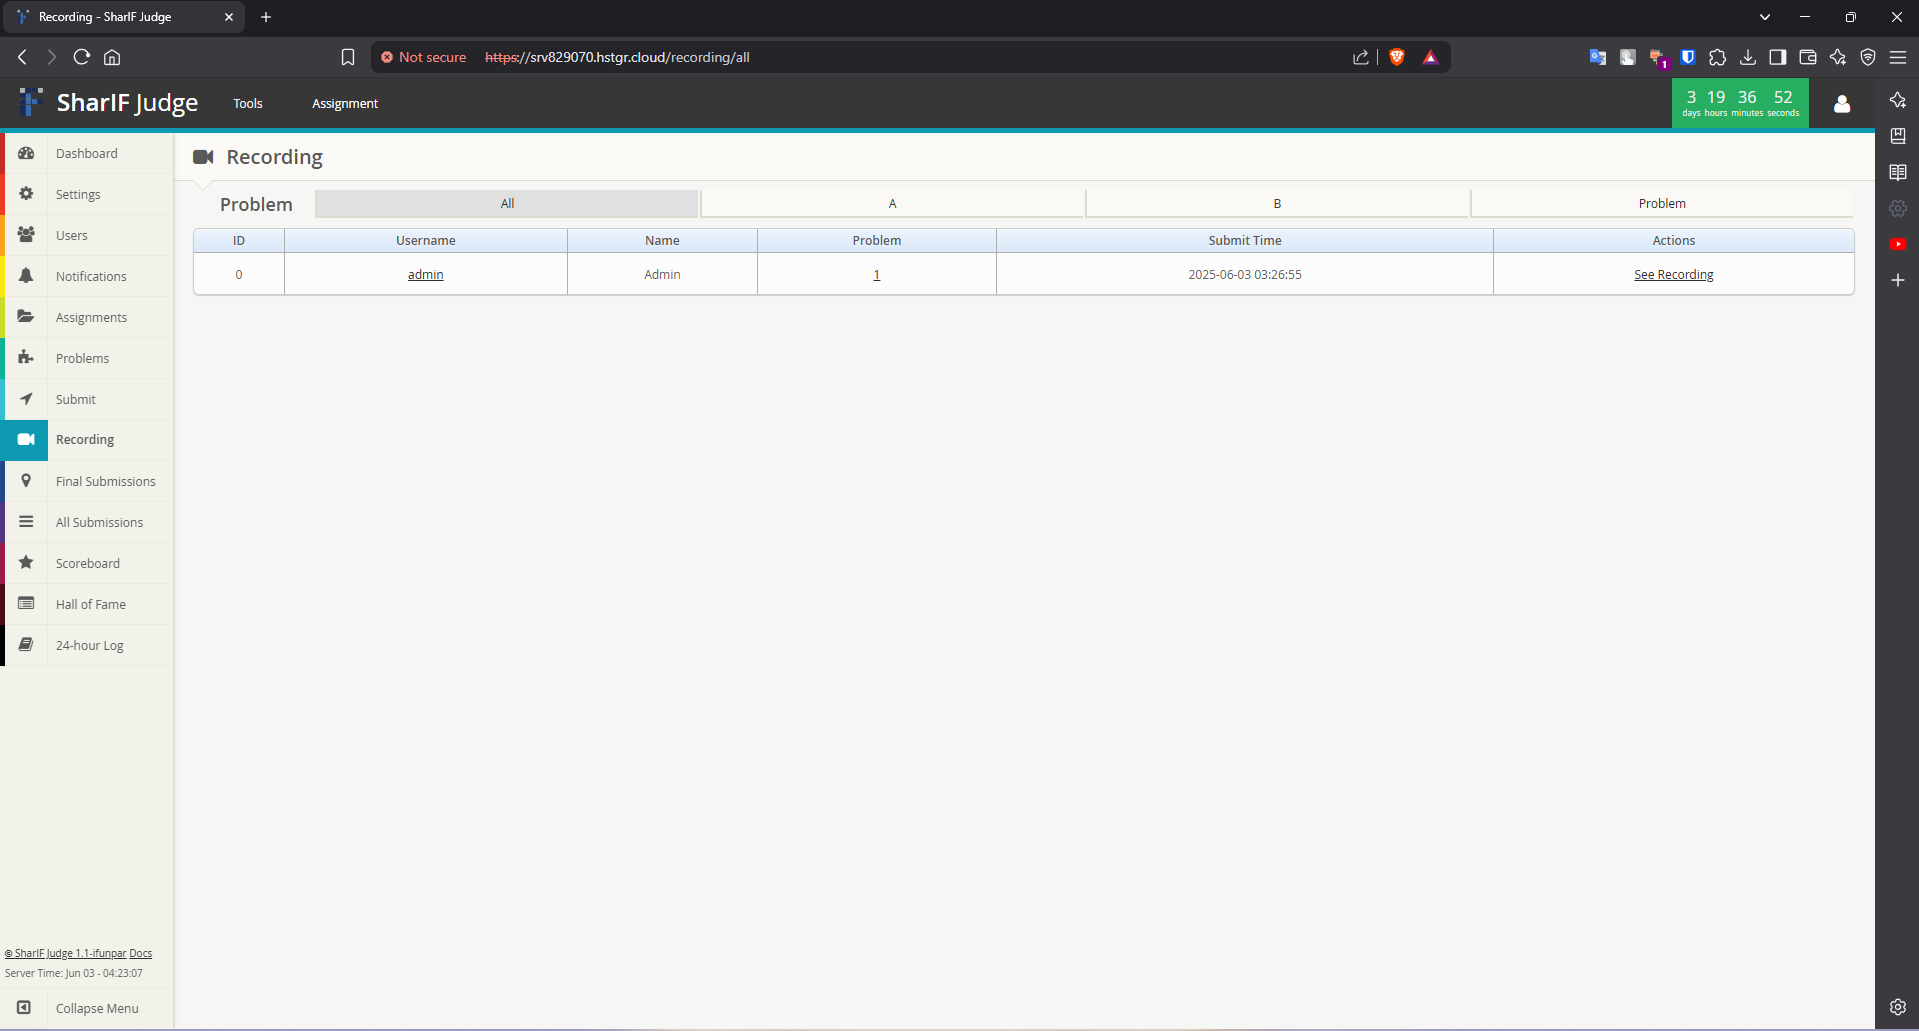
\includegraphics[width=0.85\textwidth]{views/recording_list.png}
    \caption{Halaman Daftar Rekaman}
    \label{fig:hasil:recording_list}
\end{figure}

\begin{figure}[H]
    \centering
    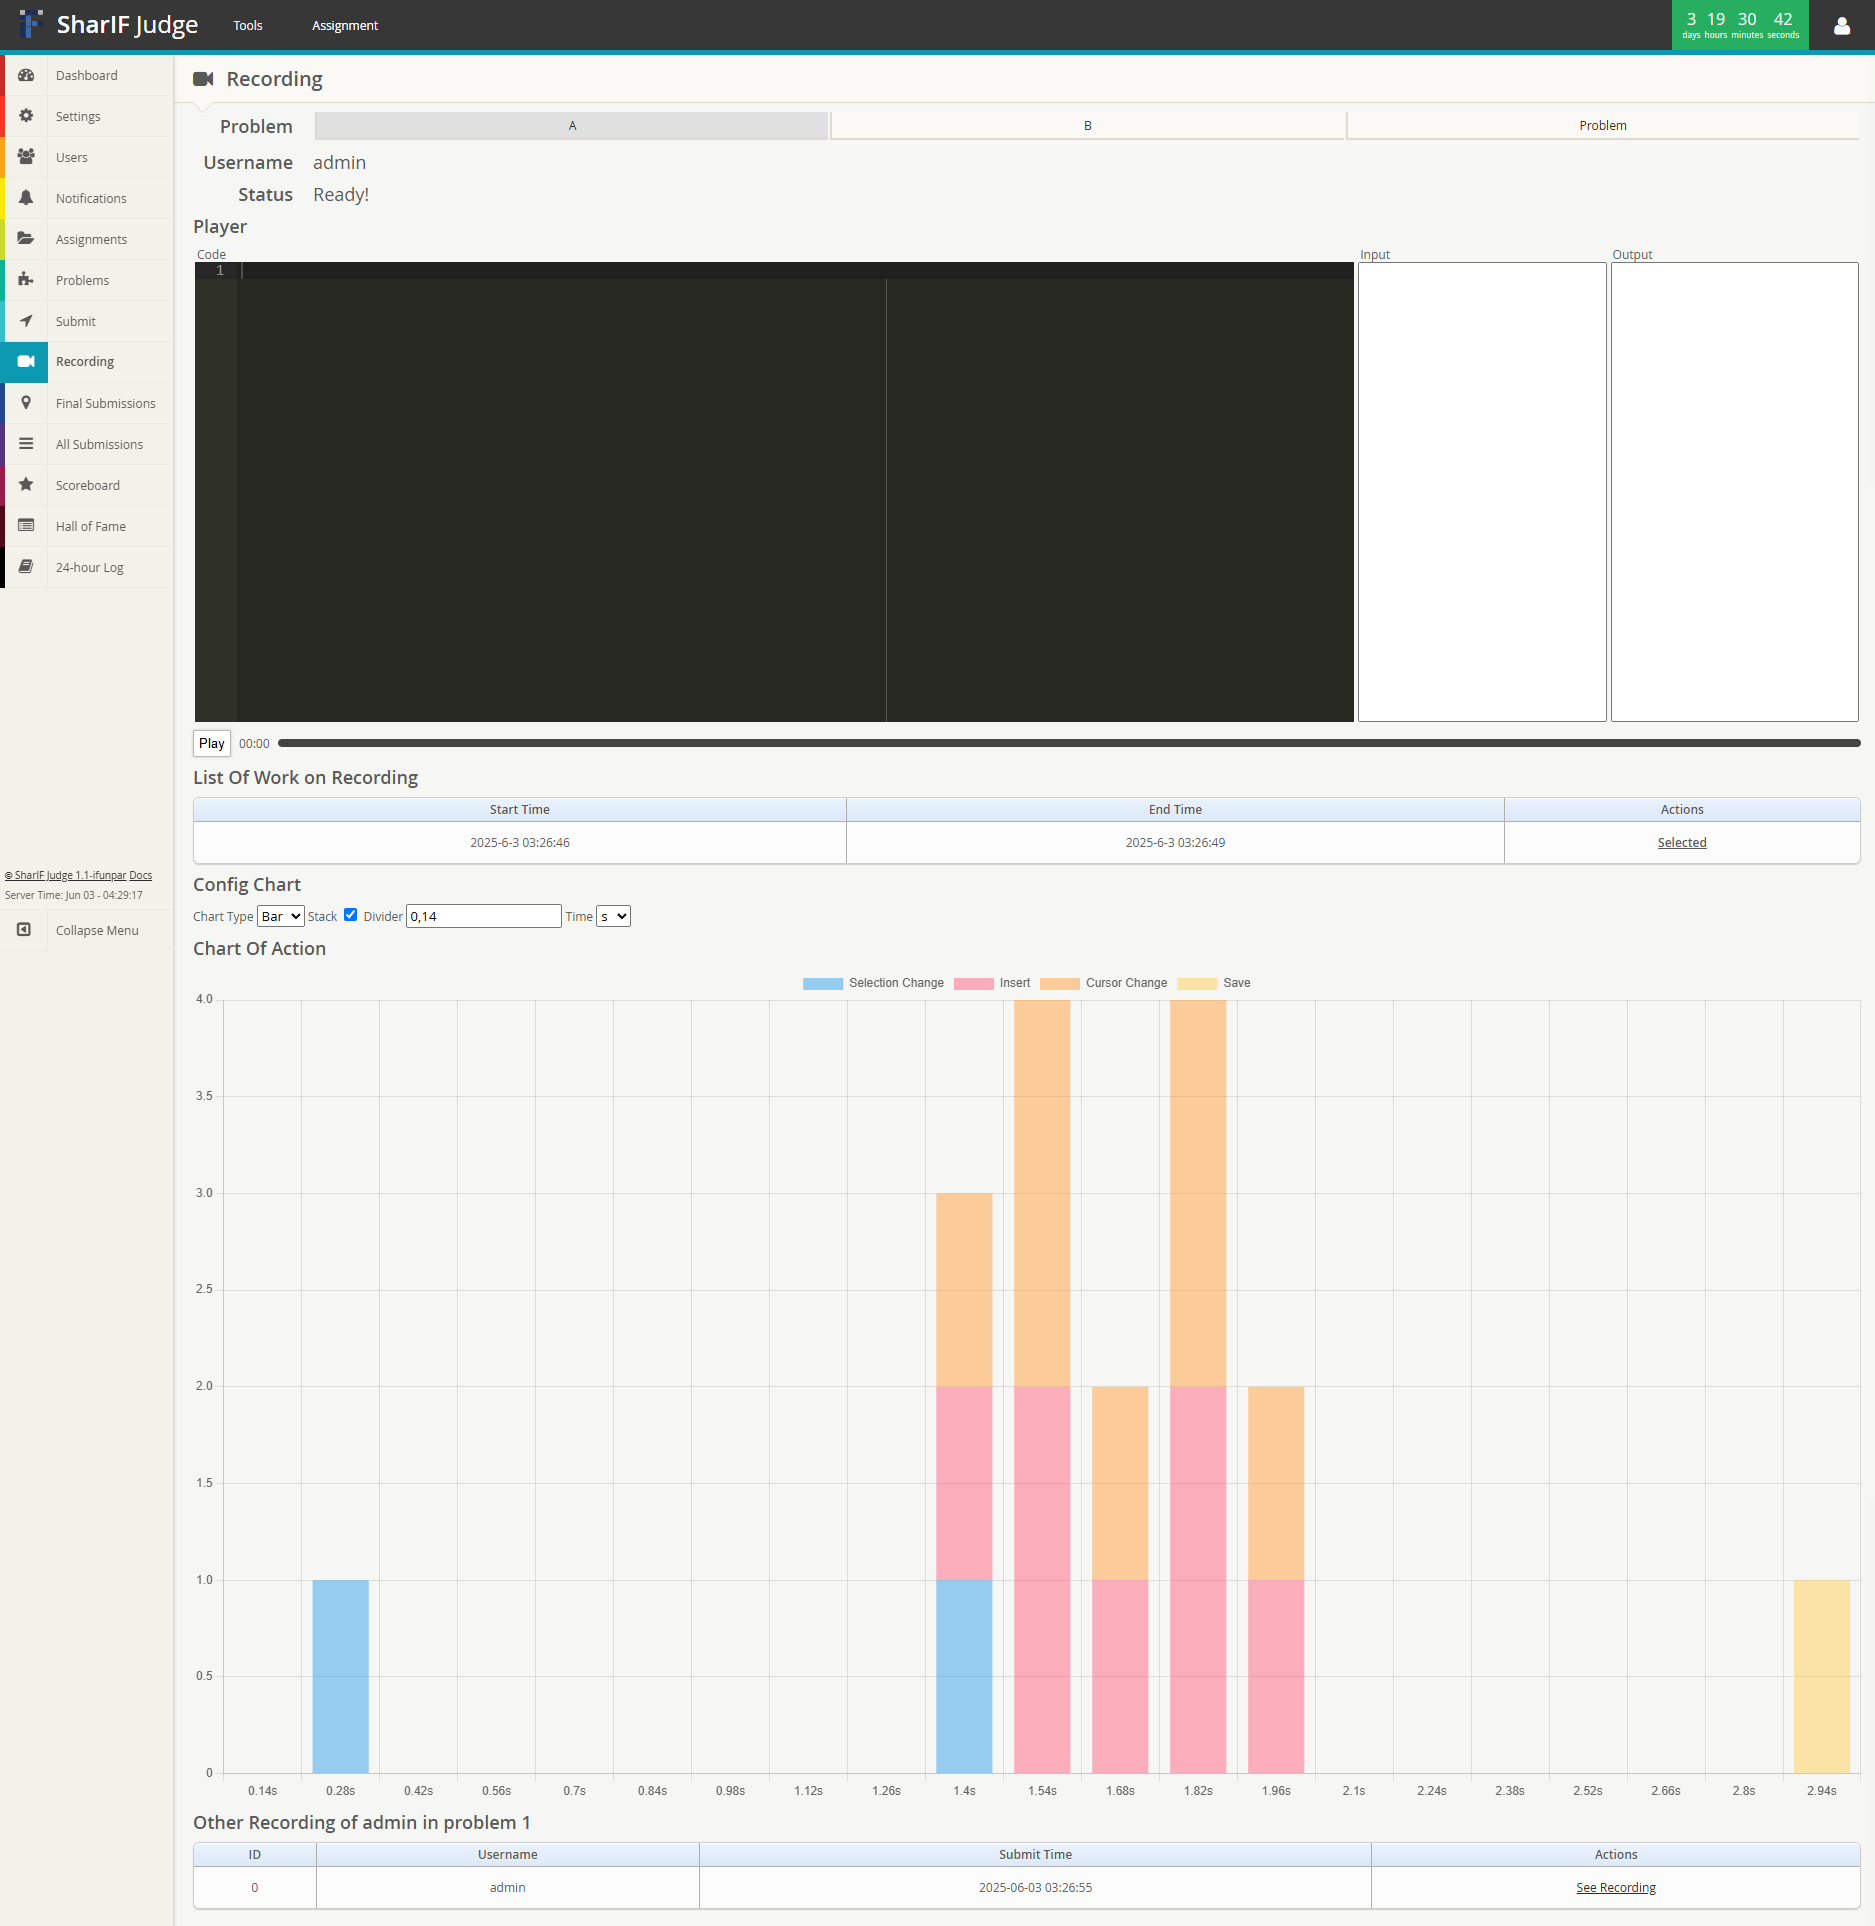
\includegraphics[width=0.85\textwidth]{views/recording.png}
    \caption{Halaman Rekaman}
    \label{fig:hasil:recording}
\end{figure}

% \lstinputlisting[language=Java, caption=MyCode.java]{./Lampiran/MyCode.java} 

